% A skeleton file for producing Computer Engineering reports
% https://kgcoe-git.rit.edu/jgm6496/KGCOEReport_template

\documentclass[CMPE]{../KGCOEReport}

% The following should be changed to represent your personal information
\newcommand{\classCode}{EEEE 380}  % 4 char code with number
\newcommand{\name}{Andrei Tumbar}
\newcommand{\LabSectionNum}{1}
\newcommand{\LabInstructor}{Dr.\ Moon}
\newcommand{\TAs}{Karen Chen}
\newcommand{\exerciseNumber}{6}
\newcommand{\exerciseDescription}{Dynamic Logic}

\usepackage{tikz}
\usepackage{circuitikz}
\usepackage{multirow}
\usepackage{titlesec}
\usepackage{float}
\usepackage{lmodern}
\usepackage{siunitx}
\usepackage{subcaption}
\usepackage{graphicx}
\usepackage[usestackEOL]{stackengine}
\usepackage{scalerel}
\usepackage[T1]{fontenc}
\usepackage{amsmath}


\def\code#1{\texttt{#1}}

\begin{document}
    \maketitle
    \section*{Abstract}

	In this exercise, the behaviour of dynamic logic circuits was investated. Unlike
	in static logic where voltage on any given node will have a direct path to ground or
	the supply voltage, dynamic circuits will charge capacitors which will share charge
	across nodes even when disconnected from the supply voltage. These circuits are
	subject to degredation overtime in the form of leakage current and parasitic
	capacitance. This lab specifically looked at the domino circuit which implements 
	the function $F = AB$.

    \section*{Basic Domino Logic Gate}
    
	The domino logic gate in question will have two inputs \code{A} and \code{B} as
	well as a \code{CLK} signal. A pulse sweep was used to control these inputs to show
	the response of the dynamic circuitry with all combinations of inputs.
    
    \begin{figure}[h!]
       \centering
       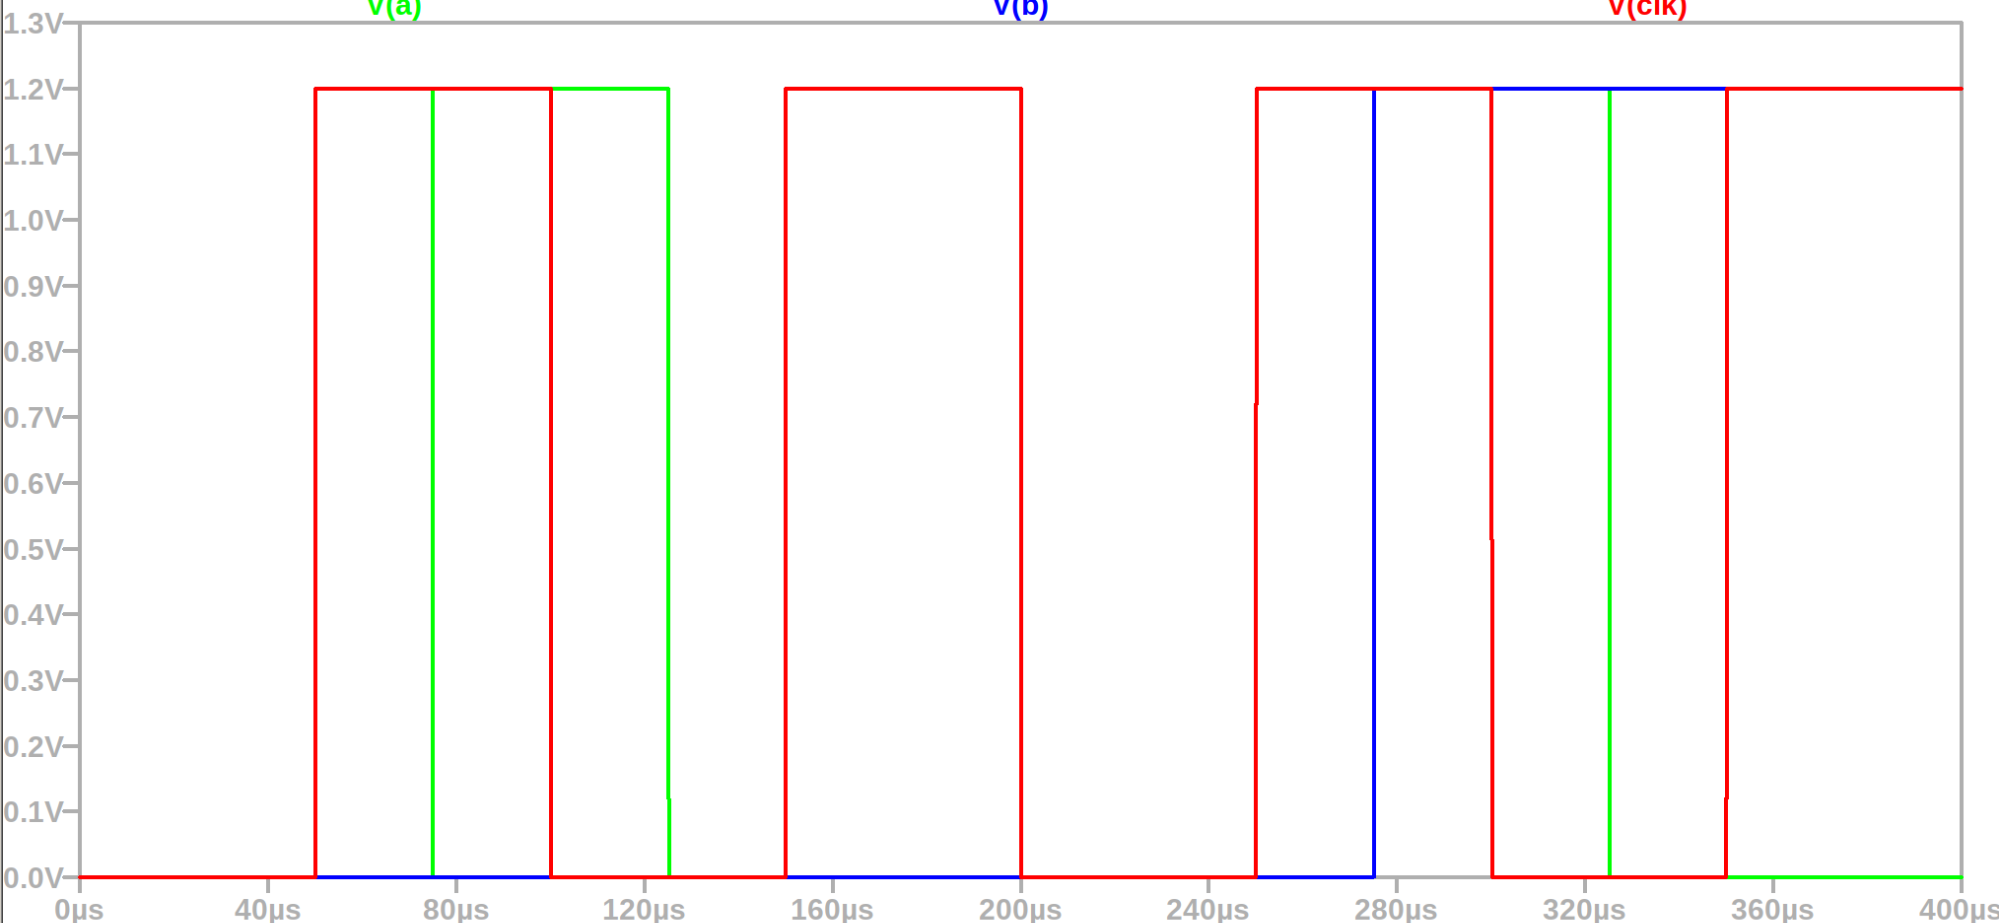
\includegraphics[width=5.5in]{img/domino_inputs.png}
       \caption{Domino logic inputs}
       \label{fig:inputs}
	 \end{figure}

	We can see in Figure \ref{fig:inputs} the only time this circuit should output a high
	logic signal is when all three signals are high. This only occurs between
	\SI{270}{\micro\s} and \SI{300}{\micro\s}. The basic domino logic gate will not model
	the capacitance at the NMOS drains for the \code{A} and \code{B} nodes. This will not
	properly model the charge sharing that will be seen in the real circuit.
    
    \begin{figure}[h!]
       \centering
       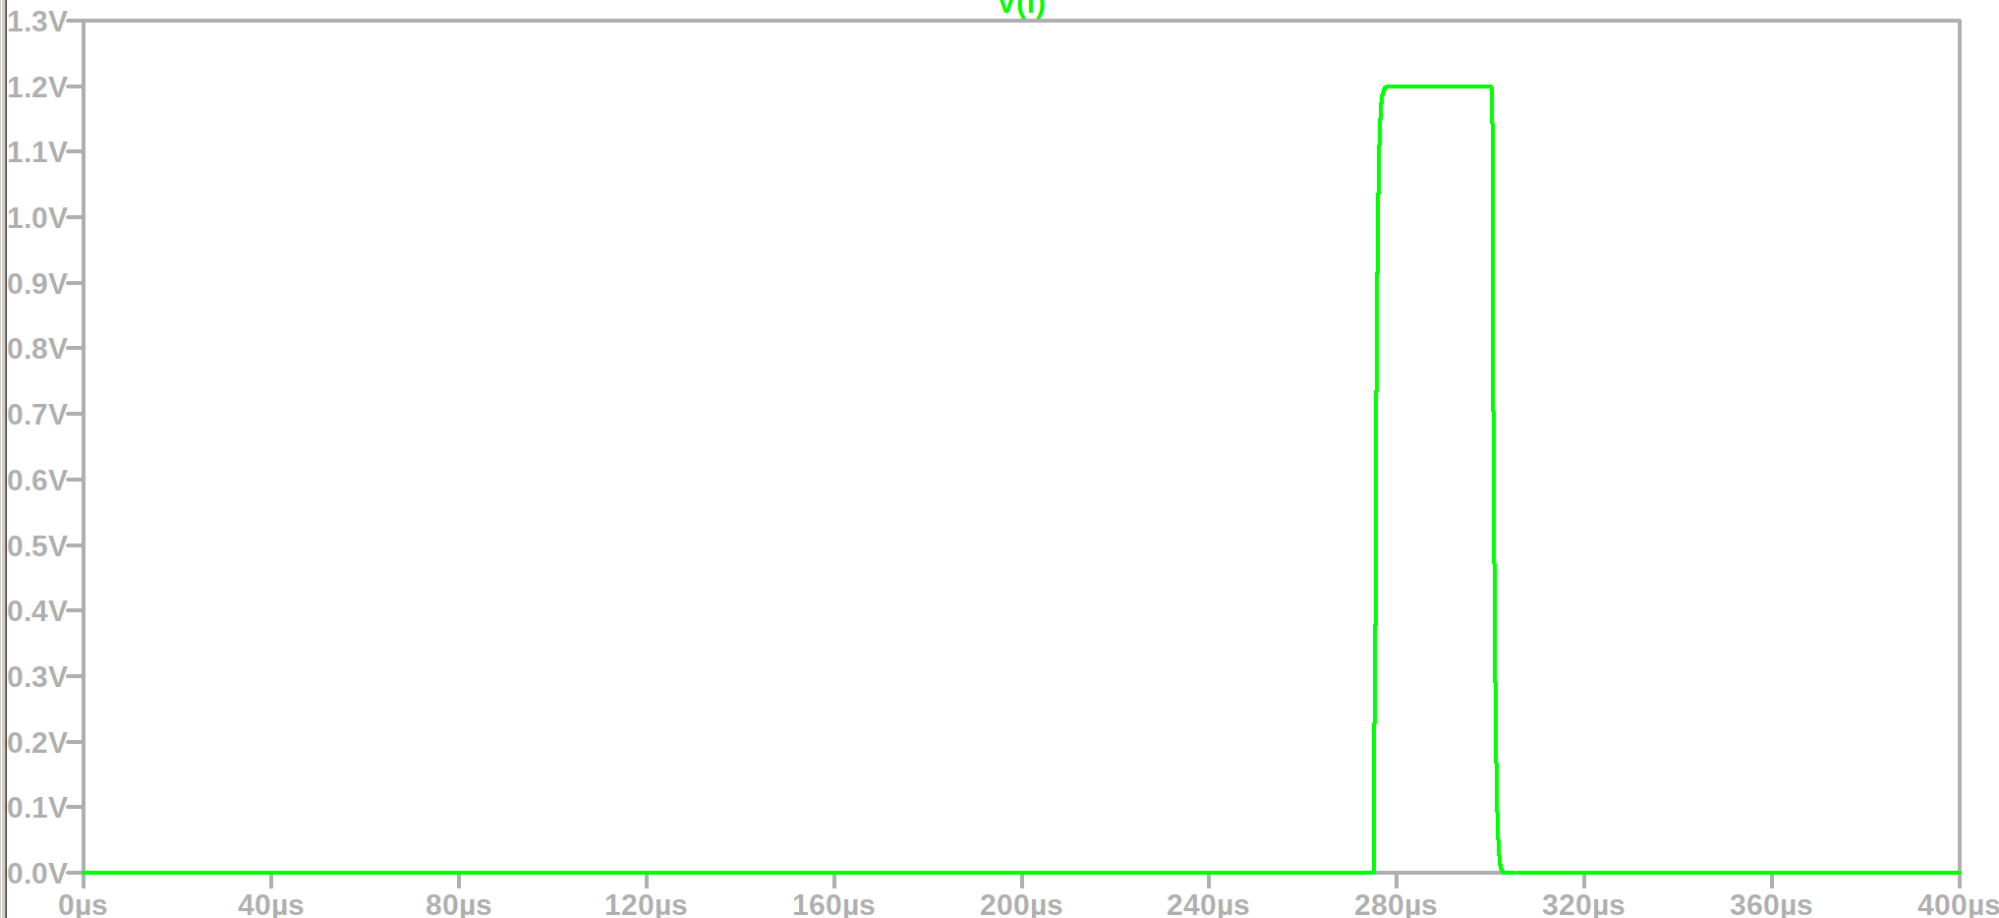
\includegraphics[width=5.5in]{img/basic_domino.png}
       \caption{Basic domino logic circuit simulated results}
       \label{fig:basic}
	 \end{figure}
	 
	 \pagebreak

	Looking at the results of simulating the basic dynamic logic circuit in Figure
	\ref{fig:basic}, we can see the circuit will undergo the expected bevahiour.

	\section*{Domino Logic with Charge Sharing}
	
	When the capacitance of the NMOS drains is modeled in LT-Spice, we can see that 
	the output logic will not keep the same behaviour.

	\begin{figure}[h!]
       \centering
       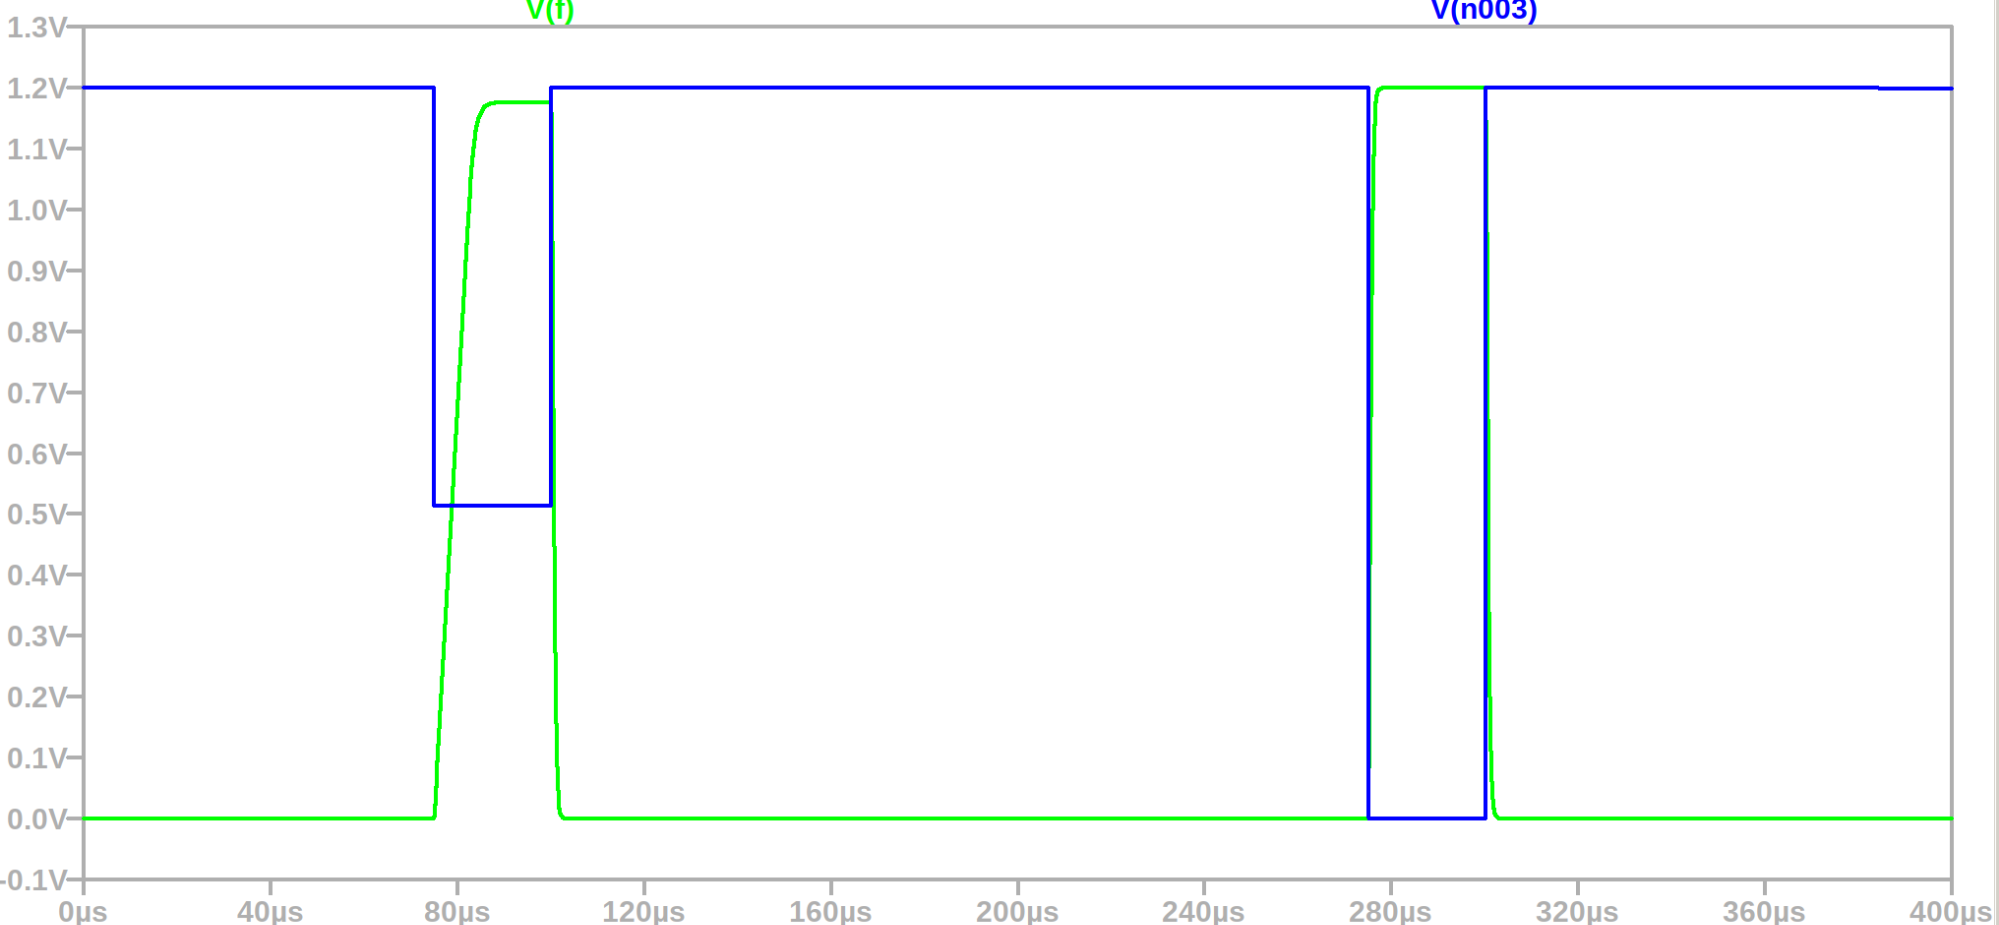
\includegraphics[width=5.5in]{img/basic_domino_charge_share.png}
       \caption{Simulated basic domino logic with charge sharing}
       \label{fig:charge_share}
	 \end{figure}

	We can see in Figure \ref{fig:charge_share} that the voltage at the inverter input
	will drop when only the \code{CLK} and \code{A} nodes are high. This is because the
	charge stored on the capacitor connected to the inverter input node will split its
	charge between itself and the capictor on the drain of the \code{A} NMOS device.
	The voltage supply is disconnected from this node as the \code{CLK} signal is high
	which keeps the pull-up network off.\\

	When the inverter input undergoes charge sharing, its voltage drops to
	\SI{0.515}{\volt}. This matches the calculated value of \SI{.514}{\volt} found
	during the prelab. When the inverter input node drops below the threshold voltage
	the output node is sent to high. This is why the output glitch occurs.

	\section*{Domino Logic with Keeper PMOS}

	To solve the issue above, an extra device is added to connect the inverter input
	to a voltage source when it would otherwise be spliting its capacitance across other
	nodes. To do this the output of the circuit is connected to a PMOS in the pull-up
	network. This will connect the inverter input to the voltage supply when output of
	the circuit is low. In this case the inverter input is high meaning its charge could
	be split across another node.

	\begin{figure}[h!]
       \centering
       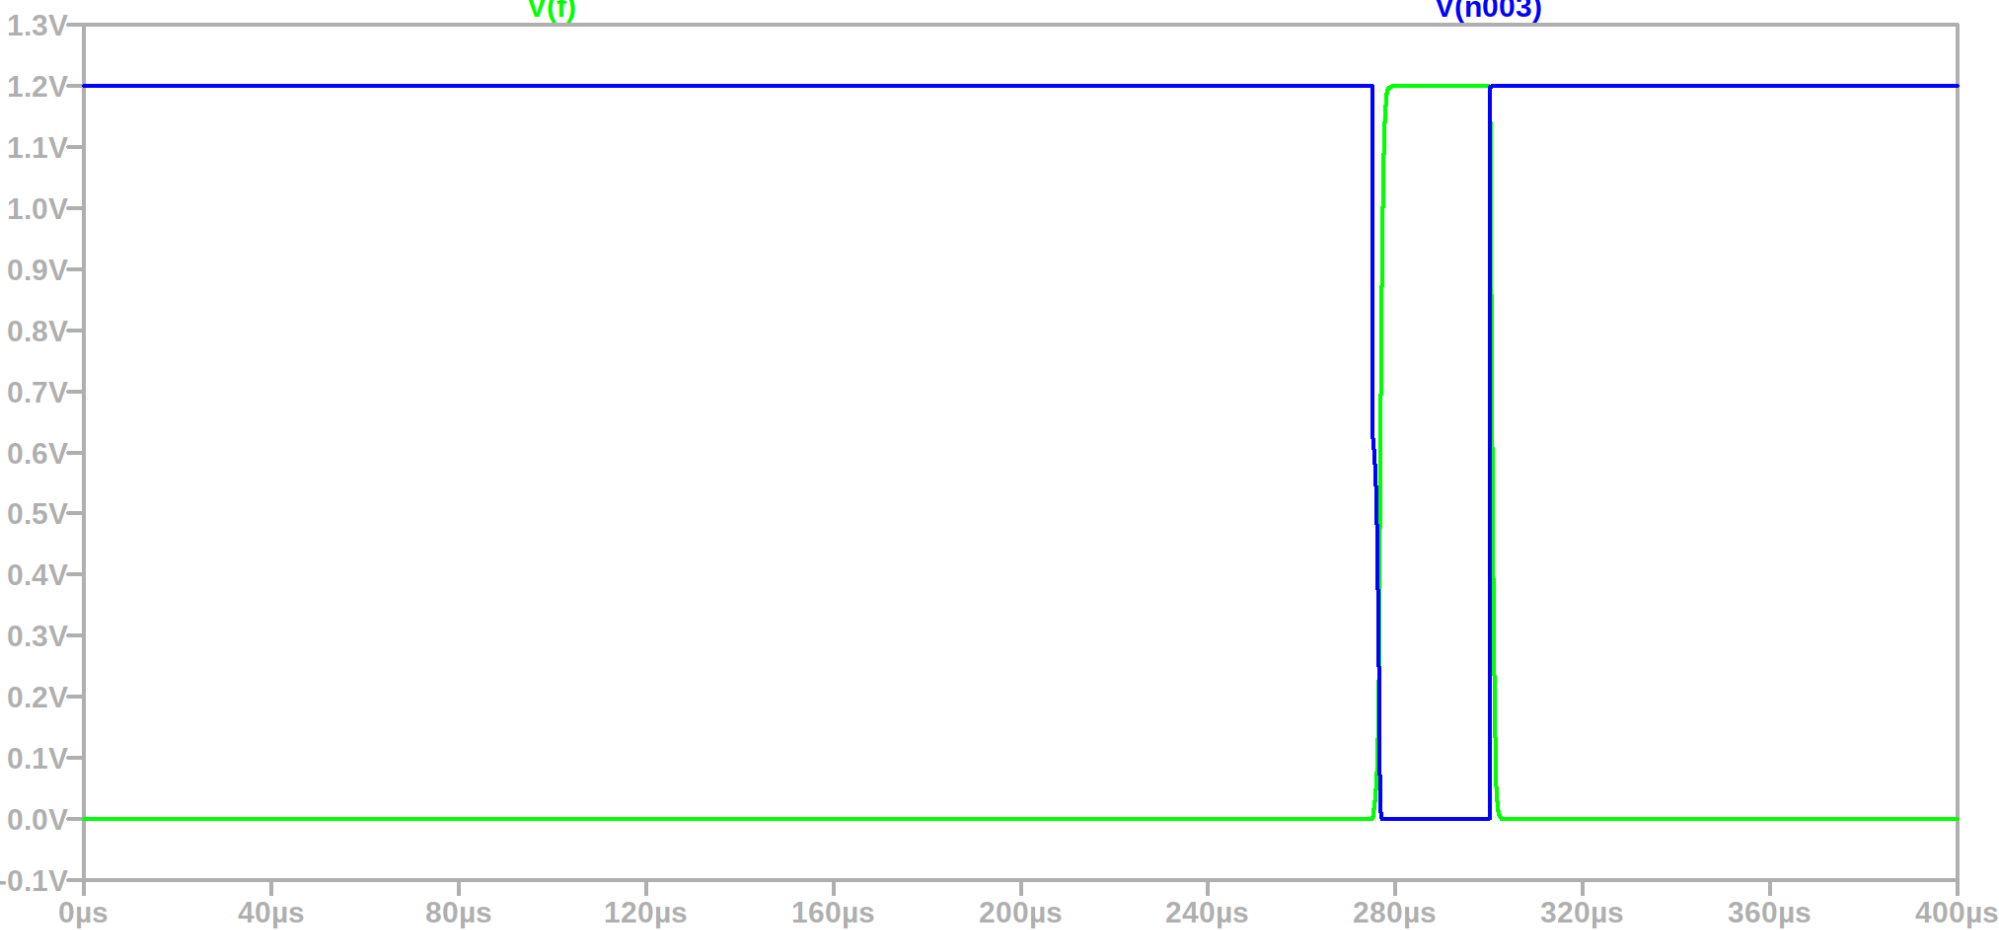
\includegraphics[width=5.5in]{img/enhanced_domino.png}
       \caption{Simulated enhanced domino logic with PMOS keeper}
       \label{fig:enhanced}
	 \end{figure}

	Comparing the simulated results of Figure \ref{fig:enhanced} to those in Figure
	\ref{fig:charge_share}, we can see that the charge sharing glitch is eliminated.
	The logic output returns to the expected output which is identical to that in the
	basic domino logic circuit shown in Figure \ref{fig:basic}. The worst case voltage
	on the inverter input will never drop below supply voltage of \SI{1.2}{\volt} with
	the PMOS keeper device. Without the keeper, this voltage will drop to
	\SI{0.515}{\volt}.

	\section*{Conclusion}

	This laboratory exercise looked at the bevaviour properties of the dynamic logic
	circuitry. The logical response of the basic domino circuit implementing the $F=AB$
	function showed expected results. When parasitic capacitance was modeled in the
	input node drains, we saw a glitch when the PMOS network was off and the voltage
	on the input of the inverter was split across another node in the pull-down network.
	To solve this glitch, a keeper PMOS was connected in parallel to the pull-up network
	which connected the inverter input to a voltage supply when the output of the circuit
	was low.

\end{document}
